\section{San Nikolos Dibar}\label{san-nikolos-dibar}

Tags: Personaggio Leggendario Creatore: Lorenzo Ispirazione: San Nicola
di Bari

\section{Nikolos Dibar}\label{nikolos-dibar}

\begin{center}\rule{0.5\linewidth}{0.5pt}\end{center}

\begin{figure}
\centering
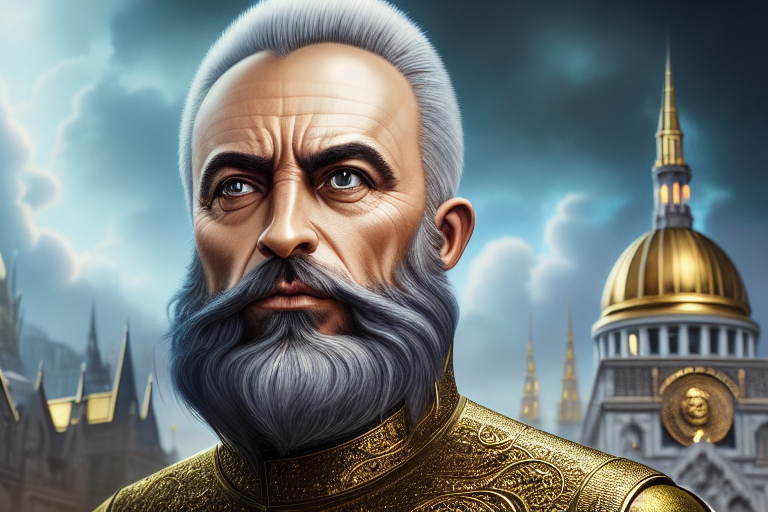
\includegraphics{uomo-di-30-anni-con-barba-e-capellimarroni-sf-intricate-artwork-masterpiece-ominous-matte-paint.png}
\caption{uomo-di-30-anni-con-barba-e-capellimarroni-sf-intricate-artwork-masterpiece-ominous-matte-paint.png}
\end{figure}

Informazioni Generali

Età: 65

Anno di nascita: 1347-1412

Paese di nascita: Pandosia

Razza: Umano

Relazioni: San venerato a Pandosia e nella regione occidentale di
Valtara

Alleati:

Nemesi:

Possedimenti importanti:

\begin{center}\rule{0.5\linewidth}{0.5pt}\end{center}

\subsection{1. Descrizione Generale}\label{descrizione-generale}

\begin{center}\rule{0.5\linewidth}{0.5pt}\end{center}

\begin{figure}
\centering
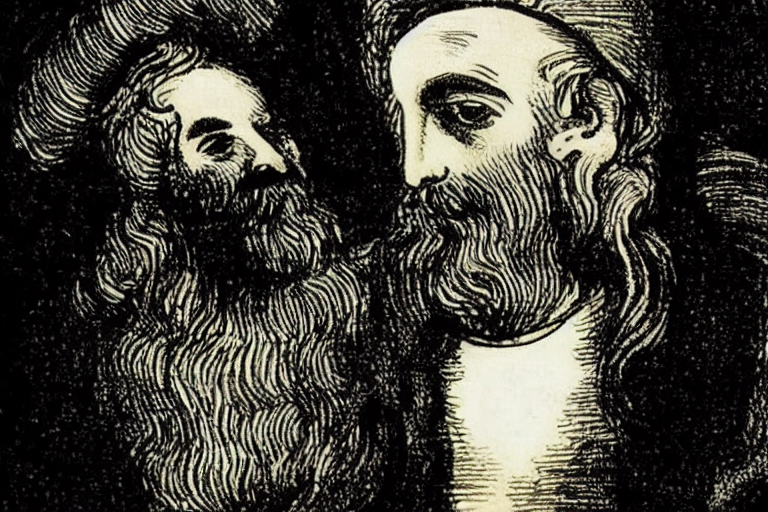
\includegraphics{san-nicolos-dibar-era-un-uomo-di-straordinaria-presenza-con-lineamenti-che-evocavano-saggezza-e-gen.png}
\caption{san-nicolos-dibar-era-un-uomo-di-straordinaria-presenza-con-lineamenti-che-evocavano-saggezza-e-gen.png}
\end{figure}

Nikolos Dibar è una figura leggendaria e venerata nella città di
Pandosia per la sua straordinaria vita da avventuriero e la sua
generosità verso gli orfani e i meno fortunati. Il titolo ``San''
attribuito a Nicolos Dibar riconosce il suo impatto eccezionale sulla
comunità e il suo status quasi mitico.

\begin{quote}
``I panittiaddri i San Nicolos'' - filastrocca popolare
\end{quote}

\subsection{2. Biografia}\label{biografia}

\begin{center}\rule{0.5\linewidth}{0.5pt}\end{center}

Nikolos Dibar nacque in una modesta casa rurale nelle campagne di
\href{Pandosia\%2028129d9d5ac7448d98387dc4262c4704.md}{Pandosia}
nell'anno 1347. Fin dalla giovane età, dimostrò un talento eccezionale
per le arti magiche e il combattimento. All'età di 16 anni, intraprese
la sua vita da avventuriero, dopo aver difeso un villaggio vicino da una
banda di briganti.

Da quel momento, Nikolos divenne noto come un potente stregone
guerriero, unendo le arti magiche e la forza fisica in modo unico. Le
sue avventure lo portarono in terre remote e misteriose, anche al di
fuori di Valtara. Dopo ogni avventura, che poteva durare anche diversi
mesi, Nikolos faceva ritorno alla sua città natale, dove donava i grandi
tesori trovati ai suoi concittadini.

Nikolos Dibar visse una vita lunga e avventurosa, ma alla fine si ritirò
dalla vita da avventuriero e si stabilì a Pandosia. Morì in pace nella
sua casa nel 1412, all'età di 65 anni, circondato dall'amore e dalla
gratitudine della comunità che aveva aiutato e ispirato per tutta la
vita.

La sua eredità continua a vivere attraverso i templi, i monumenti e le
celebrazioni in suo onore a Pandosia. Nikolos Dibar è ricordato come un
simbolo di altruismo e determinazione, un esempio di come una singola
persona possa cambiare il destino di molti attraverso la gentilezza e
l'azione coraggiosa. La sua vita e il suo impatto rimarranno una parte
indelebile della storia di Pandosia e continueranno a ispirare le
generazioni future.

\subsection{3. Carriera}\label{carriera}

\begin{center}\rule{0.5\linewidth}{0.5pt}\end{center}

Le storie di Nikolos Dibar narrano di un avventuriero coraggioso e
potente che univa le arti magiche e la forza fisica in modo
straordinario. Era conosciuto come un potente stregone guerriero e
queste sono alcune delle sue avventure più celebri:

\textbf{1. La Caccia al Drago d'Ebano}: Nikolos Dibar divenne famoso per
aver affrontato un terribile Drago d'Ebano. La bestia oscura aveva
terrorizzato i villaggi circostanti per generazioni. Nikolos, con la sua
magia e la sua abilità nella spada, sfidò il drago in un combattimento
epico che durò 2 giorni, alla fine dei quali lo sconfisse grazie al suo
incredibile coraggio.

\textbf{2. La Ricerca del Calice di Smeraldo}: Nikolos intraprese
un'ardua ricerca attraverso la foresta dei Giganti per trovare il mitico
Calice di Smeraldo, un artefatto antico di potere inestimabile.
Attraversando insidie come trappole mortali e spiriti viziati, Nikolos
alla fine recuperò il calice e lo donò alla città di Pandosia, portando
prosperità e pace.

\subsection{4. Personalità}\label{personalituxe0}

\begin{center}\rule{0.5\linewidth}{0.5pt}\end{center}

Nikolos Dibar era una figura straordinaria, non solo per le sue abilità
magiche e il suo coraggio in battaglia, ma soprattutto per la sua
personalità altruista e generosa. Credeva fermamente che donare agli
altri non solo fosse un atto di compassione, ma che elevasse anche il
suo spirito, permettendogli di condividere le gioie delle sue avventure
con gli altri. Era un uomo di cuore gentile, la cui umiltà era
sorprendente considerando le sue imprese eroiche. Nikolos aveva un'aura
di calma e compassione che attirava le persone verso di lui, e spesso si
metteva in pericolo per aiutare chiunque fosse in difficoltà. La sua
dedizione alla causa dei meno fortunati e il suo desiderio di diffondere
la speranza erano contagiosi, ispirando coloro che lo conoscevano a
compiere atti di gentilezza simili. La sua personalità luminosa e la sua
convinzione profonda nell'importanza di condividere la propria fortuna e
le proprie avventure con gli altri sono rimaste parte indelebile della
sua leggenda a Pandosia.

\subsection{5. Coinvolgimenti in eventi
recenti}\label{coinvolgimenti-in-eventi-recenti}

\begin{center}\rule{0.5\linewidth}{0.5pt}\end{center}

\href{Untitled\%20Database\%209a5498962e7a40fc8064d94e70ceaf1c.csv}{Untitled
Database}

\subsection{6. Scheda personaggio}\label{scheda-personaggio}

\begin{center}\rule{0.5\linewidth}{0.5pt}\end{center}

\href{Info\%20PG\%2009adae9699d34141ab440aa1617355d5.csv}{Info PG}

\subsubsection{Statistiche e abilità}\label{statistiche-e-abilituxe0}

\begin{center}\rule{0.5\linewidth}{0.5pt}\end{center}

\href{Abilita\%CC\%80\%20f490e2858acb4949aa11fe388d4f8d75.csv}{Abilità}

\subsubsection{Lista magie}\label{lista-magie}

\subsection{A. Descrizione originale}\label{a.-descrizione-originale}

\begin{center}\rule{0.5\linewidth}{0.5pt}\end{center}
